\section{釜式反应器的物料衡算式}


\begin{frame}{釜式反应器}
    \qquad 釜式反应器是工业上应用最广泛的反应器之一。在本章中，只研究均相反应或者可按均相反应对待的多相反应问题。
    \begin{itemize}
      \item 既可以用来进行均相反应(主要是液相均相反应)，又可用于多相反应，如气液、液固、液液及气液固等反应。
      \item 在操作方式上，可以是连续反应，也可以间歇或半间歇操作。
      \item 釜内设有搅拌装置，因此可以认为反应区内反应物料的浓度均一，温度均一。
      \item 如果反应区内存在两个或两个以上的相态，则各相的反应物料组成未必相同，温度也不一定相等，这时各相间就可能存在质量传递和热量传递，这是进行多相反应时所必须考虑的问题。
    \end{itemize}
    
\end{frame}


\begin{frame}{釜式反应器的物料衡算式}
    \qquad 设在釜式反应器中进行$M$个均相反应，描述该反应系统所需要的关键组分数为$K$，$K\le M$。如果这$M$个反应均是独立的，则$K=M$。
    \\\qquad 前已假定反应器内反应物料浓度及温度处处相同，且与流出物料的相应值相等，故可取整个反应体积$V_\mathrm{r}$作控制体积。这种情况下只有时间自变量，设在时间间隔$\mathrm{d}t$内，反应器里关键组分$i$量的变化为$\mathrm{d}n_i$，如图所示，反应器进出口的物料体积流量分别为$Q_0$和$Q$，因之在时间间隔$\mathrm{d}t$内，进出反应器的关键组分量分别为$Q_0c_{i0}\mathrm{d}t$及$Qc_{i}\mathrm{d}t$，关键组分的反应量则为$\mathcal{R}_iV_\mathrm{r}\mathrm{d}t$。
    \begin{columns}[c]
        \column{9.75cm}
            根据质量守恒定律有
            $$Q_0c_{i0}\mathrm{d}t=Qc_{i}\mathrm{d}t-\mathcal{R}_iV_\mathrm{r}\mathrm{d}t+\mathrm{d}n_i$$
            若$i$为反应物，$\mathcal{R}_i$为负；反应产物的$\mathcal{R}_i$则为正。
        \column{3.75cm}
            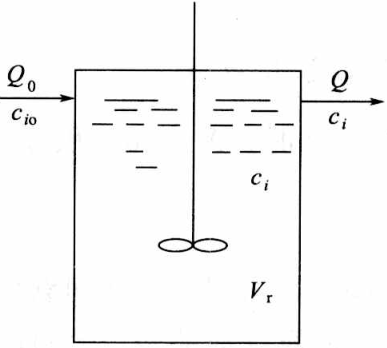
\includegraphics[height=2.5cm]{figs/fig3.1.png}
    \end{columns}
\end{frame}


\begin{frame}{釜式反应器的物料衡算式}    
    $$Q_0c_{i0}=Qc_{i}-\mathcal{R}_iV_\mathrm{r}+\mathrm{d}n_i/\mathrm{d}t \qquad (i=1,2,\cdots,K)$$
    \\这就是釜式反应器的物料衡算式，是一组常微分方程。关键组分$i$在反应器内的累积速率$\mathrm{d}n_i/\mathrm{d}t$可正可负，视具体情况而定。
    \\定态下操作的反应器，累积速率为零，
    $$Q_0c_{i0}=Qc_{i}-\mathcal{R}_iV_\mathrm{r} \qquad (i=1,2,\cdots,K)$$
    此为连续釜式反应器的物料衡算式，为一个代数方程组。
    \\如果采用间歇操作，无物料的输入与输出，即$Q_0=Q=0$，
    $$-\mathcal{R}_iV_\mathrm{r}+\mathrm{d}n_i/\mathrm{d}t=0 \qquad (i=1,2,\cdots,K)$$
    此为间歇釜式反应器的物料衡算式，为一组常微分方程。
\end{frame}